\documentclass{article}

\usepackage{graphicx}
\usepackage{tikz}
\usepackage{tikzsymbols}
\usetikzlibrary{calc,patterns,shapes.geometric}
\pagestyle{empty}
\usepackage[margin=0pt]{geometry}
\geometry{papersize={14in,12in}}

\def\centerarc[#1](#2)(#3:#4:#5){\draw[#1] ($(#2)+({#5*cos(#3)},{#5*sin(#3)})$) arc (#3:#4:#5);}

\begin{document}
	\begin{figure}
		\centering
		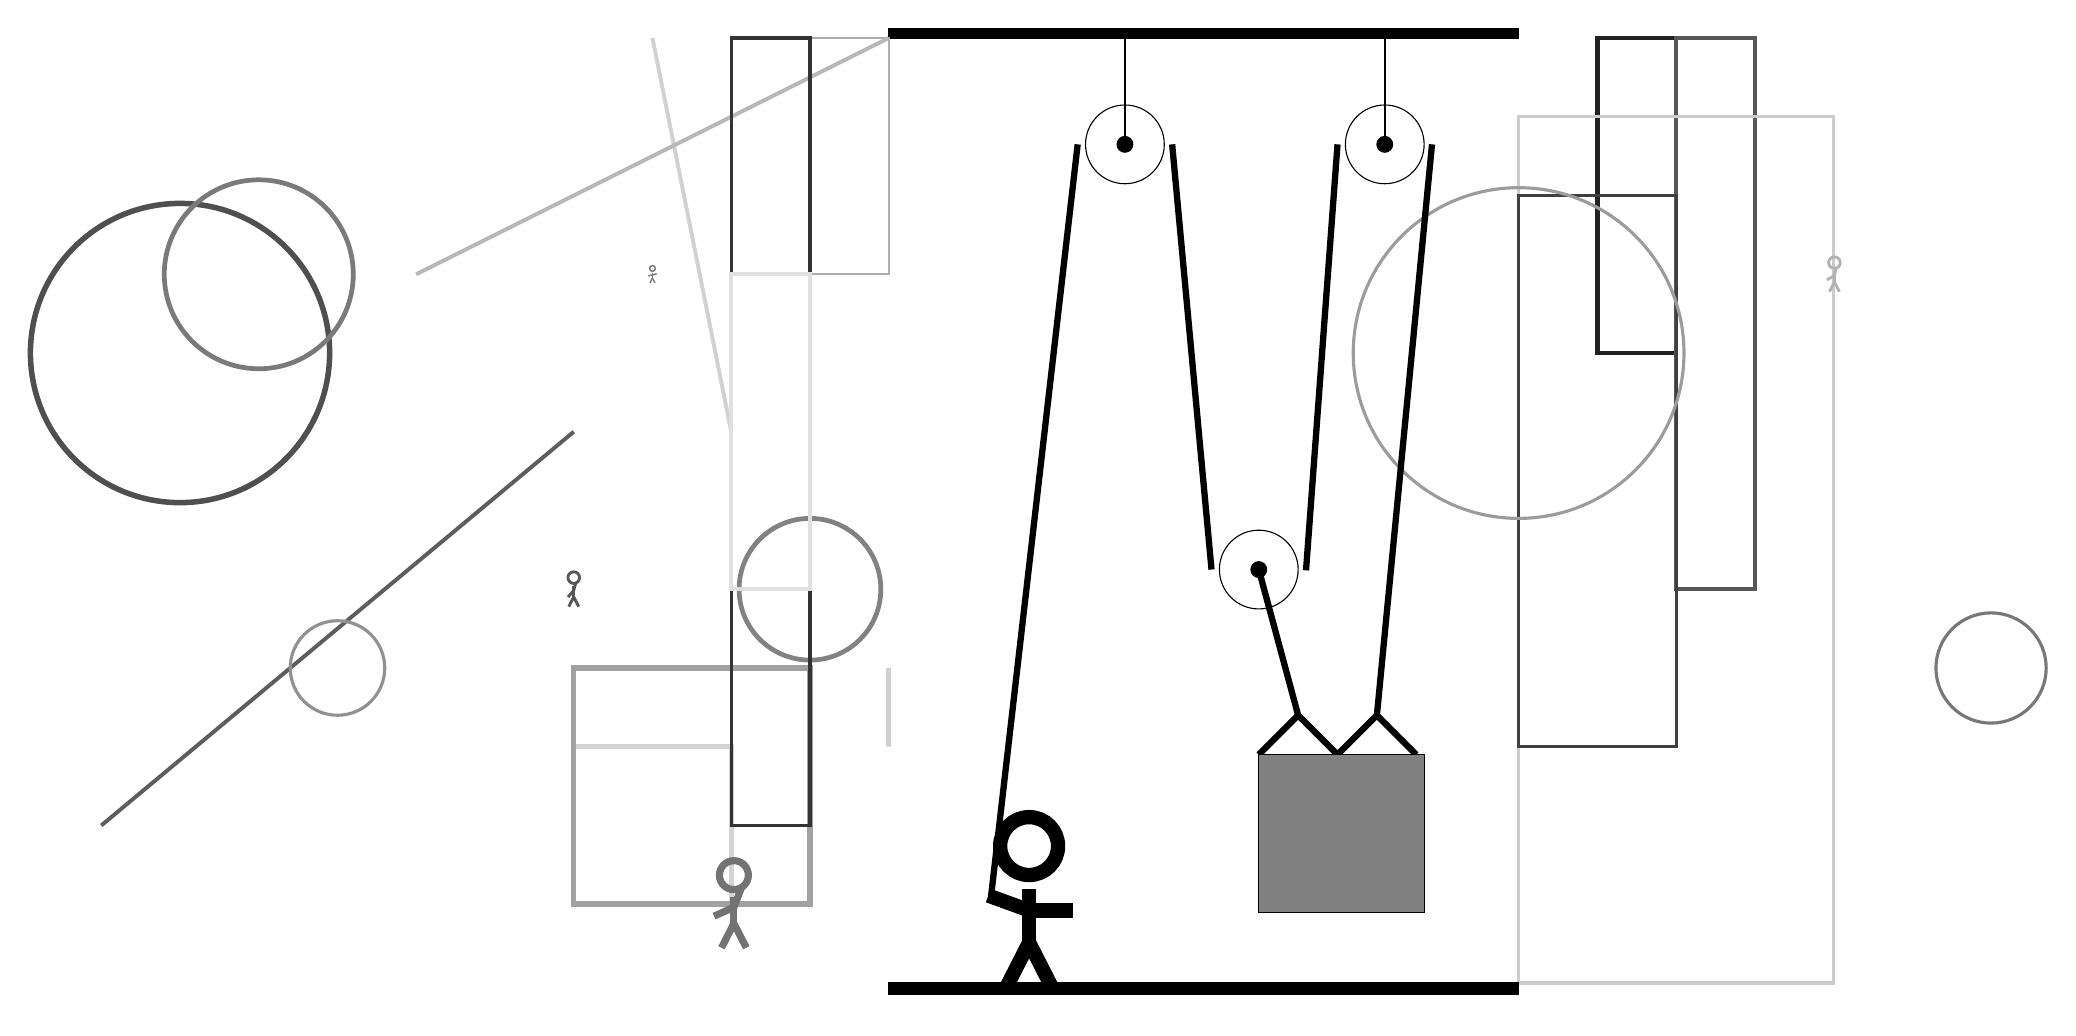
\begin{tikzpicture}
			%%%%% START %%%%%
			
			\draw[fill=black] (-2, 9) rectangle (6, 9.125);
			
			\draw (1, 7.65) circle (0.5);
			\draw[fill=black] (1, 7.65) circle (0.1);
			\draw[thick] (1, 7.65) -- (1, 9);
			
			\draw[line width=0.3mm, color=black!32] (-4, 6) rectangle (-2, 9);
			
			\draw[line width=0.4mm, color=black!83] (8, 6) rectangle (8, 8);
			\draw[line width=0.6mm, color=black!87] (8, 9) rectangle (7, 5);
			\draw[line width=0.5mm, color=black!63](-6, 4) -- (-12, -1);
			
			\draw[line width=0.5mm, color=black!66] (8, 2) rectangle (9, 9);
			
			\draw [line width=0.7mm, color=black!69](-11, 5) circle (1.9);
			\draw[line width=0.4mm, color=black!20] (6, -3) rectangle (10, 8);
			\draw[line width=0.4mm, color=black!75] (8, 7) rectangle (6, 0);
			\draw [line width=0.4mm, color=black!43](-9, 1) circle (0.6);
			
			\draw [line width=0.4mm, color=black!39](6, 5) circle (2.1);
			
			\draw[line width=0.5mm, color=black!69] (-3, -1) rectangle (-3, -2);
			
			\draw[line width=0.6mm, color=black!17] (-4, -2) rectangle (-6, 0);
			\draw[line width=0.7mm, color=black!37] (-3, -2) rectangle (-6, 1);
			
			\node[line width=0.6mm, color=black!53] at (-5, 6) {\Strichmaxerl[1][14][15]};
			\node[line width=0.2mm, color=black!55] at (-4, -2) {\Strichmaxerl[5][24][69]};
			\draw [line width=0.6mm, color=black!49](-3, 2) circle (0.9);
			
			\node[line width=0.4mm, color=black!30] at (10, 6) {\Strichmaxerl[2][30][78]};
			\draw[line width=0.5mm, color=black!18](-5, 9) -- (-4, 4);
			\draw[line width=0.5mm, color=black!28](-2, 9) -- (-8, 6);
			\draw[line width=0.4mm, color=black!80] (-3, 9) rectangle (-4, -1);
			\draw [line width=0.4mm, color=black!53](12, 1) circle (0.7);
			
			\draw[line width=0.5mm, color=black!12] (-3, 2) rectangle (-4, 6);
			\draw[line width=0.6mm, color=black!19] (-2, 1) rectangle (-2, 0);
			\draw [line width=0.6mm, color=black!52](-10, 6) circle (1.2);
			\node[line width=0.6mm, color=black!66] at (-6, 2) {\Strichmaxerl[2][49][75]};
			\draw[line width=0.6mm, color=black!67] (8, 2) rectangle (8, 2);
			
			\draw (4.3, 7.65) circle (0.5);
			\draw[fill=black] (4.3, 7.65) circle (0.1);
			\draw[thick] (4.3, 7.65) -- (4.3, 9);
			
			\draw (2.7, 2.25) circle (0.5);
			\draw[fill=black] (2.7, 2.25) circle (0.1);
			
			\draw[line width=0.8mm]  (2.7, -0.1) -- (3.2, 0.4) -- (3.7, -0.1) -- (4.2, 0.4) -- (4.7, -0.1);
			\draw[fill=black!50] (2.7, -0.1) rectangle (4.8, -2.1);
			
			\draw[line width=0.8mm](-0.7, -1.9) -- (0.4, 7.65);
			\centerarc[line width=0.8mm](1, 7.65)(0:180:0.6);
			\draw[line width=0.8mm](1.6, 7.65) -- (2.1, 2.25);
			\centerarc[line width=0.8mm](2.7, 2.25)(180:370:0.6);
			\draw[line width=0.8mm] (3.3, 2.24) -- (3.7, 7.65);
			\centerarc[line width=0.8mm](4.3, 7.65)(0:180:0.6);
			\draw[line width=0.8mm](4.2, 0.4) -- (4.9, 7.65);
			\draw[line width=0.8mm] (3.2, 0.4) -- (2.7, 2.25);
			
			\node at (-0.2, -2) {\Strichmaxerl[10][-20][0]};
			
			\draw[fill=black] (-2, -3) rectangle (6, -3.15);
			
			%%%%% END %%%%%
		\end{tikzpicture}
	\end{figure}	
\end{document}